\documentclass[12pt]{beamer} 
% handout to collapse each frame to one page

% compres pour afficher les "ronds" dans l'en-tete sur une seule ligne
% [compress] peut peut etre aussi se mettre dans le declaration du theme
% fleqn pour mettre un numero a droite aux equations, c'est ledno pour a droite
% cette numerotation ne marche apparement pas sous beamer...

% style beamer
%\usetheme{Darmstadt}
\usetheme{Boadilla}
%\usetheme{Warsaw}
%\usetheme{Pittsburgh }
%\usetheme{Madrid}
%\usetheme{Rochester}
%\usetheme{Copenhagen}
%\usetheme{Singapore}
%\usetheme{Malmoe}
%\usetheme{Marburg}
%\useoutertheme{miniframes}
%\useoutertheme{smoothbars}
%\usecolortheme[named=seahorse]{structure} %  utiliser avec xcolor=dvipsnames dans les options de document beamer

\usepackage[english]{babel}   % Document en anglais
\usepackage[utf8x]{inputenc}  % Accents dans le source
\usepackage{ucs}
\usepackage{amsmath}
\usepackage{amsfonts}
\usepackage{amssymb}
\usepackage{stmaryrd}
\usepackage{makeidx}
%\usepackage[svgnames]{xcolor} % Pour mettre de la couleur

\usepackage{graphicx}
\usepackage{tabularx}

\usepackage{fixltx2e}

\graphicspath{ {img/} }

\usepackage{listings}
\usepackage{caption}
\usepackage{forloop}
%\usepackage{subfig}

\usepackage{color}
%\usepackage{soul}
\usepackage[normalem]{ulem}

\definecolor{black}{rgb}{0,0,0}
\definecolor{white}{rgb}{1,1,1}
\definecolor{red}{rgb}{1,0,0}
\definecolor{specialblue}{RGB}{51,51,179}

% packages style
\usepackage{pslatex}
%\usepackage{graphicx}
\usepackage{multirow}
\usepackage{fancyvrb}

\usepackage[absolute,overlay]{textpos}
\newcommand{\putat}[3]{\begin{picture}(0,0)(0,0)\put(#1,#2){#3}\end{picture}}

\usepackage[autoplay]{animate}


\usepackage{listings}
\usepackage{color}
\definecolor{keywords}{RGB}{255,0,90}
\definecolor{comments}{RGB}{60,179,113}
\lstset{language=Python,
keywordstyle=\color{keywords},
commentstyle=\color{comments}\emph,
basicstyle=\scriptsize\tt}

\usepackage{minted}
\usemintedstyle{emacs}

% \renewcommand{\theFancyVerbLine}{\sffamily
% \textcolor[rgb]{0.5,0.5,1.0}{\scriptsize
% \oldstylenums{\arabic{FancyVerbLine}}}}

% from http://tex.stackexchange.com/questions/57151/how-do-i-prevent-conflicts-between-accsupp-and-hyperref
\usepackage{accsupp}
\newcommand\emptyaccsupp[1]{\BeginAccSupp{ActualText={}}#1\EndAccSupp{}}


%default definition is: \def\theFancyVerbLine{\rmfamily\tiny\arabic{FancyVerbLine}}
\let\theHFancyVerbLine\theFancyVerbLine% don't apply our patch to hyperref's version
\def\theFancyVerbLine{\rmfamily\tiny\emptyaccsupp{\arabic{FancyVerbLine}}}

% Embed Python in Latex
% http://www.stevecheckley.co.uk/python.sty
% http://www.stevecheckley.co.uk/blog/tag/latex/
% http://www.texample.net/weblog/2008/oct/24/embedding-python-latex/
\usepackage{python}


% suppression de la barre de navigation
\setbeamertemplate{navigation symbols}{}

\setbeamertemplate{footline}{
\begin{beamercolorbox}[ht=2.5ex,dp=1.125ex,%
      leftskip=.3cm,rightskip=.3cm plus1fil]{}%
       \hfill    \small \insertframenumber/\inserttotalframenumber%
    \end{beamercolorbox}%
  }

% Customized title page
\defbeamertemplate*{title page}{Boadilla theme}[1][]{
  \begin{center}
  
\includegraphics[width=0.65\textwidth]{logos/cython.png}
  \vspace{0.1\textheight}
  
  {\usebeamerfont{title}\usebeamercolor[fg]{title}\inserttitle}\par
  {\usebeamerfont{subtitle}\usebeamercolor[fg]{subtitle}\insertsubtitle}\par
  \vspace{0.05\textheight}
  {\usebeamerfont{author}\insertauthor}\par
  %\vspace{0.02\textheight}
  \usebeamerfont{institute}\insertinstitute\par
  %\inserttitlegraphic\par
  \vspace{0.15\textheight}
  { \footnotesize\insertdate}\par
% \vspace{0.1\textheight}
  \end{center}
}
\title[]{Example with GCoptimization}
\author[K. Keraudren]{Kevin Keraudren}
\date{October 31\textsuperscript{st}, 2013}
\institute[ICL]{Imperial College London}

% image de fond
%\setbeamertemplate{background canvas}{}%{\includegraphics[width=\paperwidth,height=\paperheight]{bckgrnd.eps}}

%% \AtBeginSection[]{
%%  \begin{frame}{Outline}
%%    \small
%%    \begin{columns}
%%      \begin{column}{5cm}
%%        \tableofcontents[sections={1-4},currentsection, hideothersubsections]
%%      \end{column}
%%      \begin{column}{5cm}
%%        \tableofcontents[sections={5-8},currentsection, hideothersubsections]
%%    \end{column}
%%  \end{columns}
%% \end{frame} 
%% }
% \AtBeginSection[]{
%  \begin{frame}
%    \tableofcontents[currentsection, hideothersubsections]
% \end{frame} 
% }
\usepackage{tikz}
\usetikzlibrary{arrows,shapes}
%\usetikzlibrary{positioning}
\tikzstyle{na} =  [baseline=-.5ex]
\tikzstyle{nb}= [] % [baseline=10.5ex]

% For every picture that defines or uses external nodes, you'll have to
% apply the 'remember picture' style. To avoid some typing, we'll apply
% the style to all pictures.
\tikzstyle{every picture}+=[remember picture]

%\setbeamertemplate{footline}[frame number]

%\everymath{\displaystyle}

\begin{document}

% ------ page de titre ------
%\frame{\titlepage}[plain]
\begin{frame}[plain]
	\titlepage
\end{frame}

% ------ sommaire ------
 %[allowframebreaks]%
% \begin{frame}
% 	\tableofcontents
% \end{frame}

\begin{frame}{Cython overview}

\begin{itemize}
\item Syntax between Python and C (keyword \texttt{cdef})
\item C/C++ code automatically generated,\\
 then compiled into a Python module
\item For a speed gain, variables must be declared
\item C++ templates must be instantiated (compiled code)
\item Choose between accessing low-level C++ or a blackbox
\end{itemize}

\begin{center}
Documentation: \url{docs.cython.org}\\
\vspace{0.02\textheight}
Learn from examples:\\
scikit-learn, scikit-image, \url{github.com/amueller}
\end{center}
\end{frame}

\begin{frame}{How to?}
\begin{enumerate}
\item Organize your C/C++ code
\item Write \texttt{module.pyx}
\item Write \texttt{setup.py}
\item Build
\end{enumerate}
\end{frame}

\begin{frame}
\begin{center}
\LARGE
\textcolor{specialblue}{Example 1}

\Large

\vspace{0.1\textheight}

Interface the whole API
\end{center}
\end{frame}

\begin{frame}{Graphcut (Boykov \& Kolmogorov)}

\begin{center}
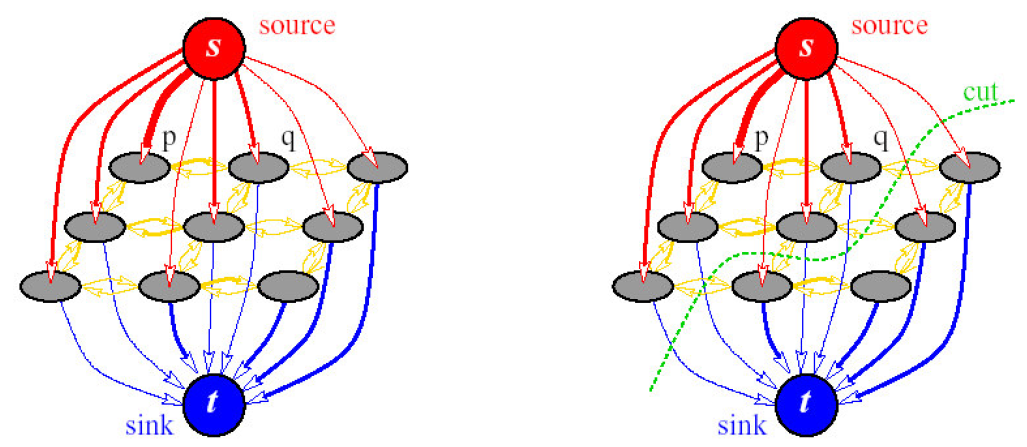
\includegraphics[width=0.75\textwidth]{graphcut.png}

\vspace{0.1\textheight}
{\large

$
 V(p,q) = \left\{ 
  \begin{array}{l l}
    \frac{1}{\|p-q\|_2}e^{ - (I_p - I_q)^2 / 2 \sigma ^ 2 } & \quad \text{if $I_p \ge I_q$}\\
    \frac{1}{\|p-q\|_2} & \quad \text{if $I_p < I_q$}\\
  \end{array} \right.
$
}
\vspace{0.05\textheight}

$\sigma$ : noise estimate
\end{center}
\end{frame}


\begin{frame}[fragile]{GCoptimisation (Boykov \& Kolmogorov)}

\small

\begin{minted}{c++}
template <typename captype,
          typename tcaptype,
          typename flowtype> class Graph {
public:
  ...
	Graph( int node_num_max, int edge_num_max,
           void (*err_function)(const char *) = NULL);
	void add_edge( node_id i, node_id j,
                   captype cap, captype rev_cap);
	void add_tweights( node_id i,
                       tcaptype cap_source, tcaptype cap_sink);
	flowtype maxflow( bool reuse_trees = false, 
                      Block<node_id>* changed_list = NULL);
	termtype what_segment( node_id i,
                           termtype default_segm = SOURCE);
  ...
}
\end{minted}
\end{frame}

\begin{frame}[fragile]{Begin your \texttt{module.pyx}}

\begin{minted}{python}

import numpy as np
cimport numpy as np

np.import_array()

ctypedef double captype
ctypedef double tcaptype
ctypedef double flowtype

\end{minted}
\end{frame}

\begin{frame}[fragile]{Declare what you need from C++}

\begin{minted}{python}
cdef extern from "graph.h":
    cdef cppclass Graph[captype,tcaptype,flowtype]:
        Graph( size_t, size_t ) 
        size_t add_node(size_t)
        void add_edge(size_t,size_t,captype,captype)
        void add_tweights(size_t,tcaptype,tcaptype)
        flowtype maxflow()
        int what_segment(size_t)
\end{minted}
\end{frame}

\begin{frame}[fragile]{Create your Python class}
\footnotesize
\begin{minted}{python}
cdef class PyGraph:
    # hold a C++ instance which we're wrapping
    cdef Graph[captype,tcaptype,flowtype] *thisptr    
    def __cinit__(self, size_t nb_nodes, size_t nb_edges):
        self.thisptr = new Graph[captype, 
                      tcaptype, flowtype](nb_nodes,nb_edges)
    def __dealloc__(self):
        del self.thisptr
\end{minted}
\end{frame}

\begin{frame}[fragile]{Create your Python class}
\footnotesize
\begin{minted}{python}
    def add_node(self, size_t nb_nodes=1):
        self.thisptr.add_node(nb_nodes)
    def add_edge(self, size_t i, size_t j, 
                          captype cap, captype rev_cap):
        self.thisptr.add_edge(i,j,cap,rev_cap)
    def add_tweights(self, size_t i, 
                        tcaptype cap_source, tcaptype cap_sink):
        self.thisptr.add_tweights(i,cap_source,cap_sink)
    def maxflow(self):
        return self.thisptr.maxflow()
    def what_segment(self, size_t i):
        return self.thisptr.what_segment(i)
\end{minted}
\end{frame}

\begin{frame}[fragile]{Write \texttt{setup.py}}
\scriptsize
\begin{minted}{python}
from distutils.core import setup
from distutils.extension import Extension
from Cython.Distutils import build_ext
from numpy.distutils.misc_util import get_numpy_include_dirs

setup(
    cmdclass = {'build_ext': build_ext},
    ext_modules = [
        Extension( "graphcut", 
                   [ "graphcut.pyx",
                     "../maxflow-v3.02.src/graph.cpp",
                     "../maxflow-v3.02.src/maxflow.cpp" ],
                   language="c++",
                   include_dirs=get_numpy_include_dirs()+["../maxflow-v3.02.src"],
                  )
        ]
    )
\end{minted}

\small

And build:
\begin{minted}{bash}
python setup.py build_ext --build-temp tmp \\
                          --build-lib lib \\
                          --pyrex-c-in-temp
\end{minted}
\end{frame}

\begin{frame}[fragile]{And use it!}
\footnotesize
\begin{minted}{python}
from lib import graphcut
G = graphcut.PyGraph(nb_pixels,nb_pixels*(8+2))
G.add_node(nb_pixels)
...
print "building graph..."     
for i in range(img.shape[0]):
    for j in range(img.shape[1]):
        for a,b in neighbourhood:
            if ( 0 <= i+a < img.shape[0]
                 and 0 <= j+b < img.shape[1] ):
                    dist = np.sqrt( a**2 + b**2 )
                    if img[i,j] < img[i+a,j+b]:
                        w = 1.0/dist
                    else:
                        w = np.exp(-(img[i,j] - img[i+a,j+b])**2
                        w /= 2.0 * std**2 * dist
                    G.add_edge( index(i,j,img),
                                index(i+a,j+b,img),
                                w, 0 )
\end{minted}
\end{frame}

\begin{frame}{Result}

\begin{center}
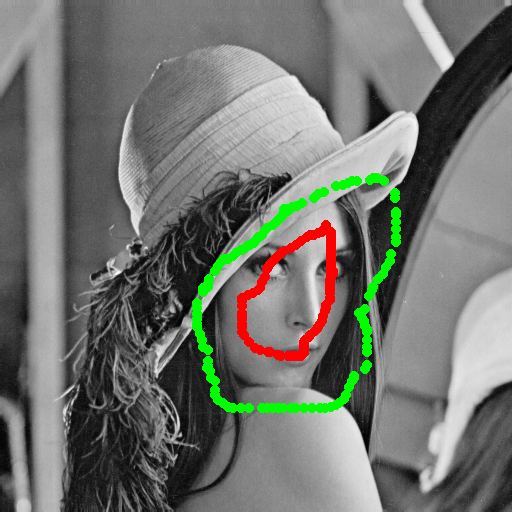
\includegraphics[width=0.45\textwidth]{initialisation.png}
\hspace{0.04\textwidth}
\includegraphics[width=0.45\textwidth]{demo/graphcut1/segmentation.png}
\end{center}

\end{frame}

\begin{frame}
\begin{center}
\LARGE
\textcolor{specialblue}{Example 2}

\Large

\vspace{0.1\textheight}

Use C++ as a blackbox
\end{center}
\end{frame}

\begin{frame}[fragile]{Declare C++ function}

\begin{minted}{python}
cdef extern from "_graphcut.h":
    void _graphcut( voxel_t*,
                   int, int,
                   double,
                   unsigned char*,
                   unsigned char* )
\end{minted}
\end{frame}
  
\begin{frame}[fragile]{And use it!}
\small
\begin{minted}{python}  
def graphcut( np.ndarray[voxel_t, ndim=2, mode="c"] img,
              np.ndarray[unsigned char, ndim=2, mode="c"] mask,
              double std ):

    cdef np.ndarray[unsigned char, 
                    ndim=2, 
                    mode="c"] seg = np.zeros( (img.shape[0],
                                               img.shape[1]),
                                              dtype='uint8')
    print "starting graphcut..."                                                                 
    _graphcut( <voxel_t*> img.data,
               img.shape[0], img.shape[1],
               std,
               <unsigned char*> mask.data,
               <unsigned char*> seg.data )
    return seg
\end{minted}
\end{frame}

\begin{frame}{Result}

\begin{center}
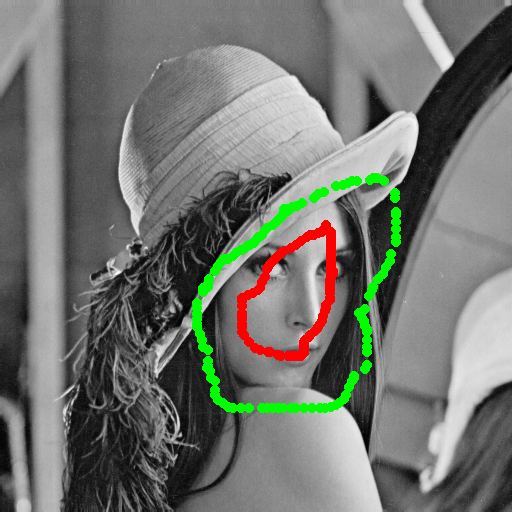
\includegraphics[width=0.45\textwidth]{initialisation.png}
\hspace{0.04\textwidth}
\includegraphics[width=0.45\textwidth]{demo/graphcut2/segmentation.png}
\end{center}

\end{frame}

\begin{frame}{Timing}

\begin{center}
\begin{minipage}{0.4\textwidth}
Example 1: 18.01s\\
Example 2: 0.37s

\vspace{0.05\textheight}

Nearly 50 times faster...
\end{minipage}
\end{center}
\end{frame}

\begin{frame}{Another result...}

\begin{center}
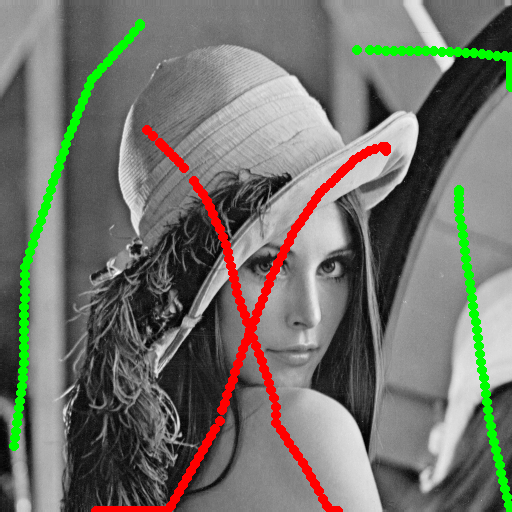
\includegraphics[width=0.45\textwidth]{initialisation2.png}
\hspace{0.04\textwidth}
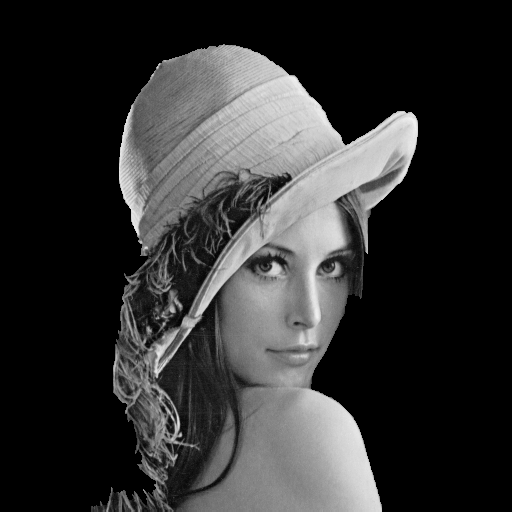
\includegraphics[width=0.45\textwidth]{demo/graphcut2/segmentation2.png}
\end{center}

\end{frame}

\begin{frame}{Conclusion}

\begin{itemize}
\item Huge speedup for a low amount of code
\item Perfect if C++ code already exists
\item Make sure your Python code is optimised (good use of \texttt{numpy})
  before using \texttt{cython}  
\end{itemize}

\vspace{0.05\textheight}

\begin{center}
\large
Examples are available for download
\end{center}
\end{frame}


\begin{frame}
\begin{center}
\LARGE
\textcolor{specialblue}{Thanks!}
\end{center}
\end{frame}

\end{document}
% ------ fin document ------
